\section{Deployment View}

This section is devoted to explain in details the physical architecture of the \textit{TrackMe} system, with mentions to the communication protocols that will be used.

%\vskip\bigskipamount

\begin{figure}[H]

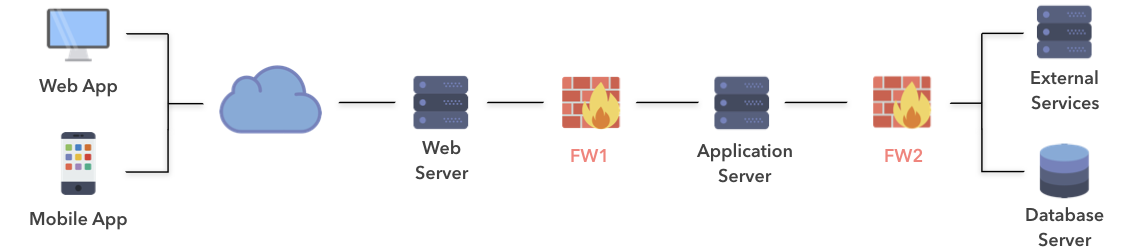
\includegraphics[scale=0.32,keepaspectratio]{./Pictures/high-level-firewall.png}
\centering
\caption{High-level architecture}

\end{figure}

First of all, two different clients are put in place: a lightweight Web application that will be accessible from any modern Web Browser and a full Mobile application with support for both iOS and Android, the two most popular mobile operating systems. The Mobile application will manage User's data through \textit{Realm}, an ODBMS which provides support for both iOS and Android. In order to have a highly maintainable system, the communication between the clients and the server will adhere to the \textit{REST} protocol, which is built on top of \textit{HTTPS}. 
The requests will be received from an \textit{Apache Web Server}, where they will be forwarded to the application server after being filtered by a firewall.
The \textit{Application Server} is the central element of the system architecture and it needs high performance, security assurance and high availability. Our engineering team found in \textit{IBM WebSphere Application Server} the product that best meets these needs. The server will run the application on the \textit{EJB} environment and it will be the only element to interact with the database. The \textit{Database Server} will be an \textit{IBM DB2}, so that when technical support is needed only a single vendor has to be contacted for both the application and database server. To enhance the security of the system, the Application Server and the Database Server are set in a demilitarized zone delimited by firewalls, in order to prevent unwanted connections.
Finally, the \textit{Application Server} needs to interact with the external service, such as . Both the map service and the call/sms service are of paramount importance for the \textit{TrackMe} system, because they provide important utility for the final users. The choice of the map service is \textit{OpenStreetMap} for its reliability and privacy. The call and sms service is entrusted to CallHub.

\begin{figure}[H]

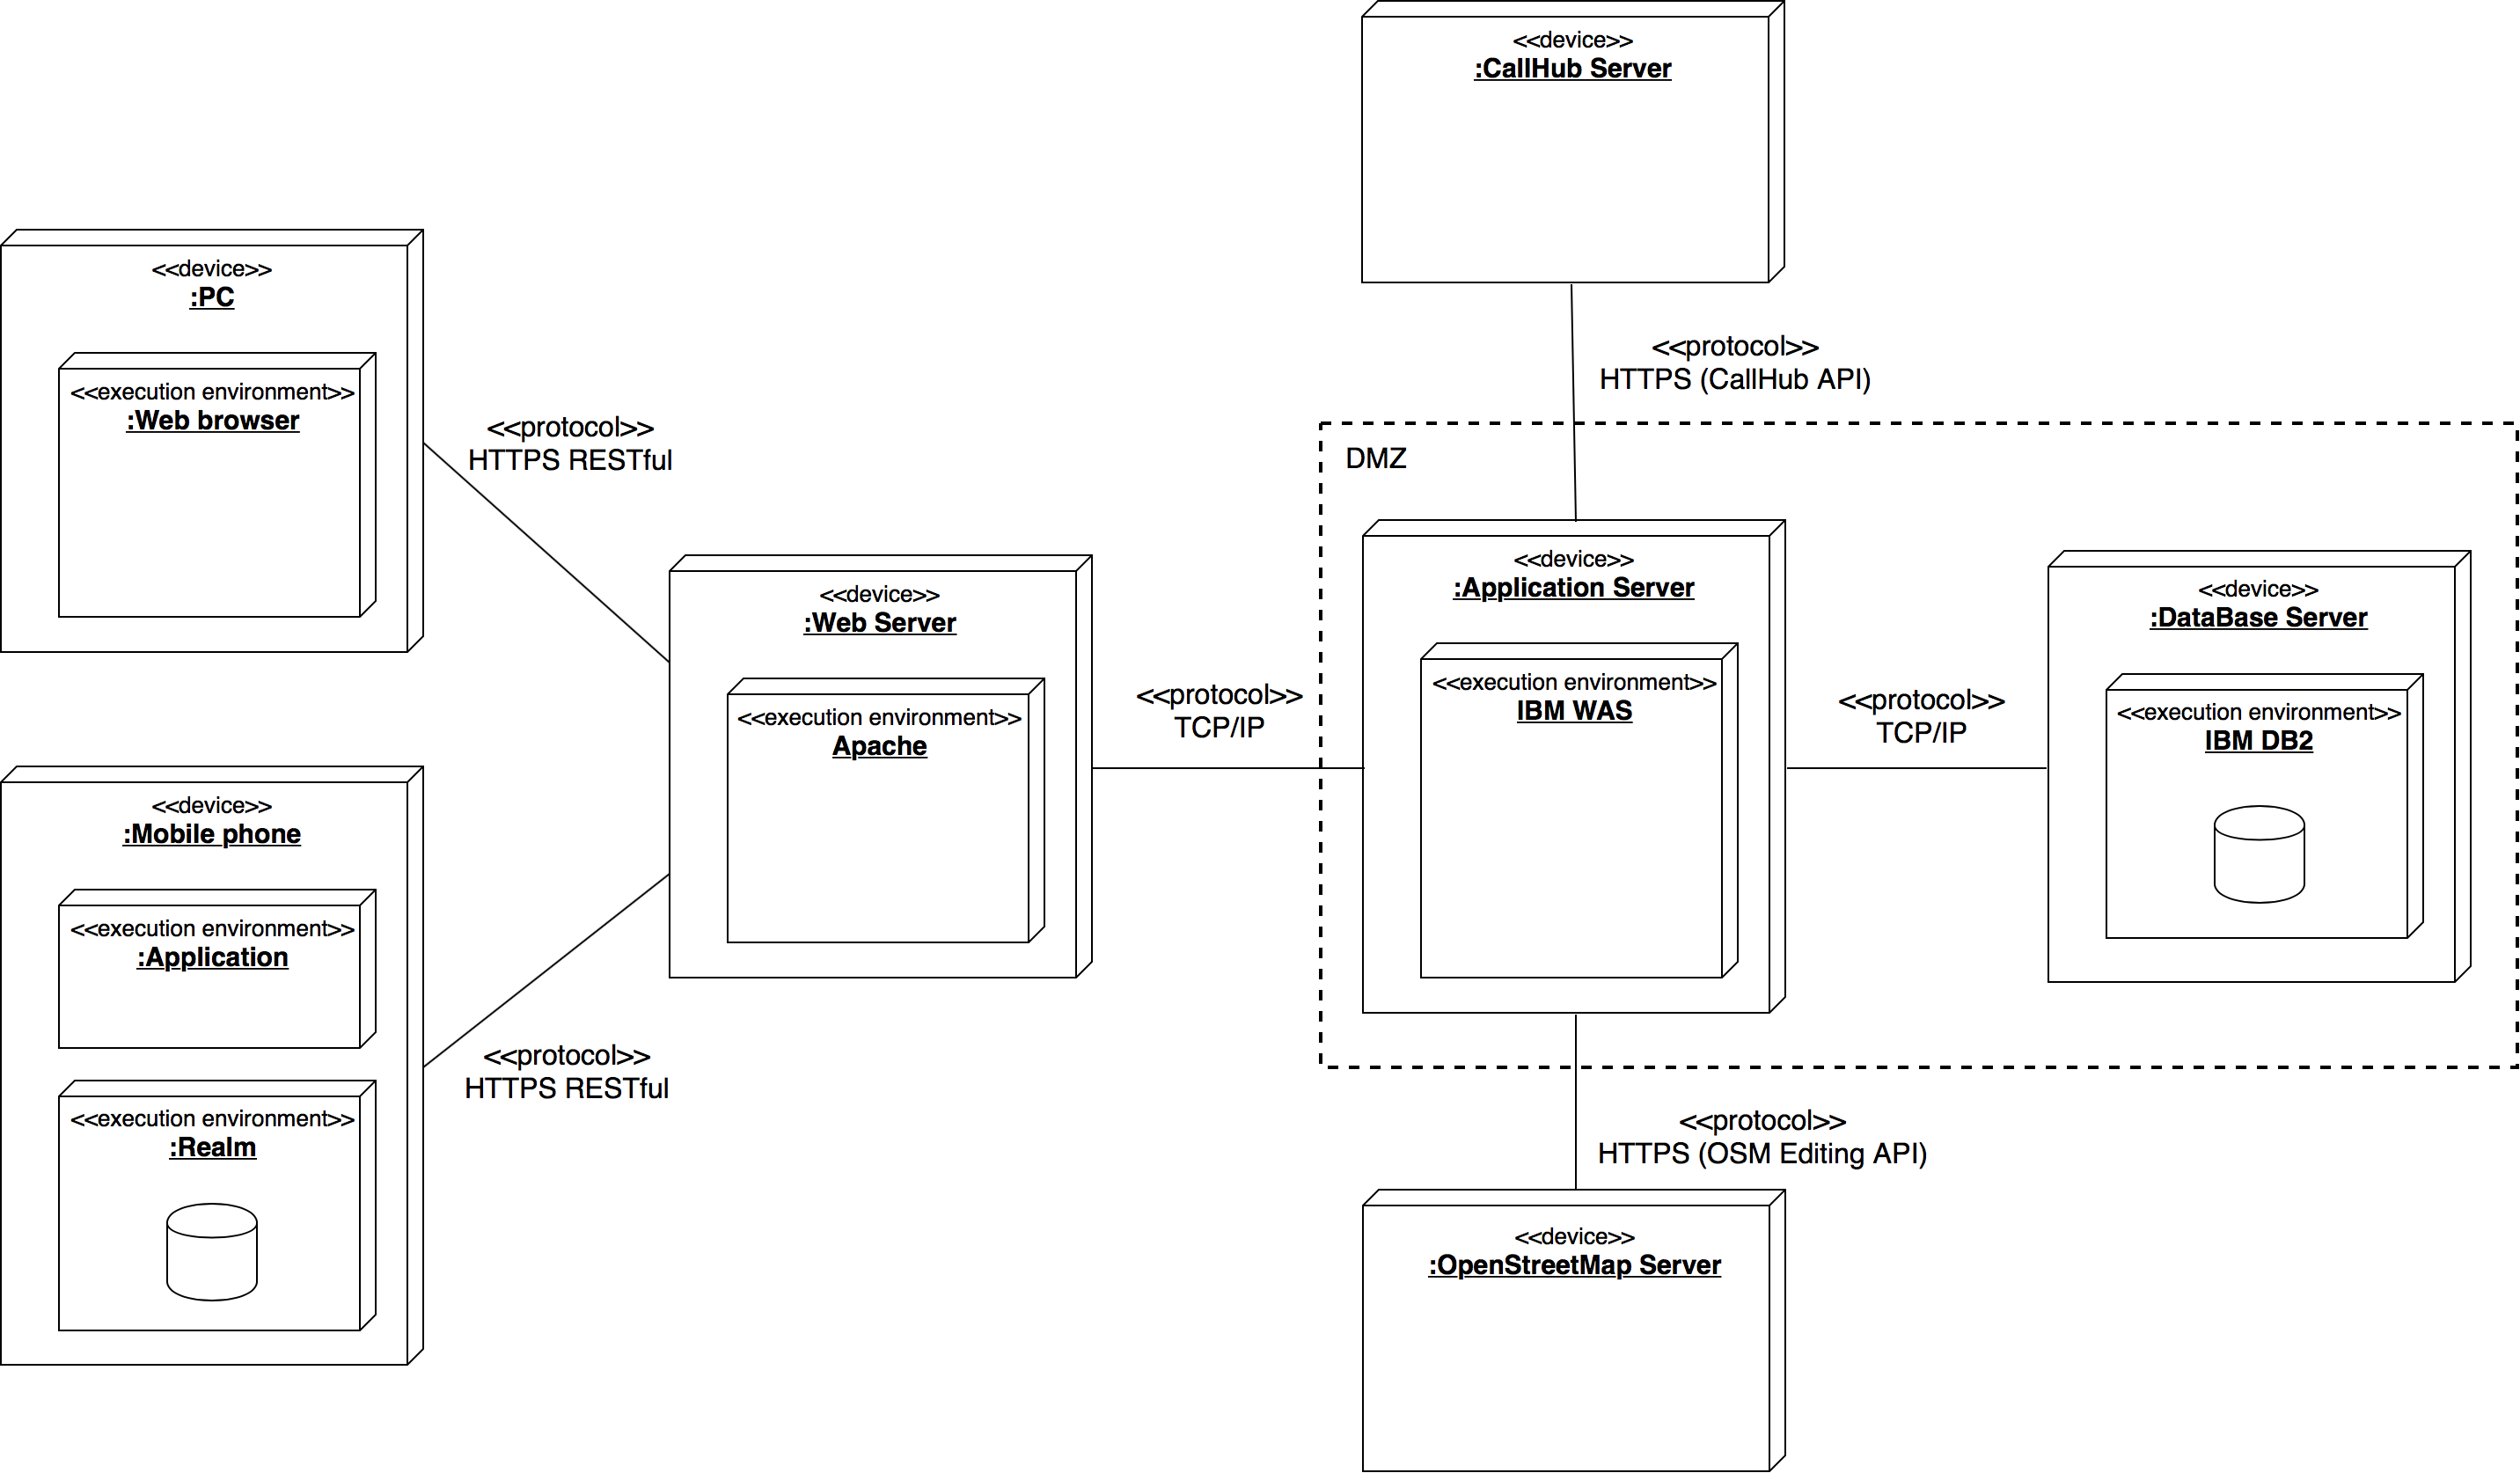
\includegraphics[scale=0.14,keepaspectratio]{./Pictures/deployment.png}
\centering
\caption{Deployment of the \textit{TrackMe} system}

\end{figure}